\subsection{Safety Artifacts}
\label{subsec:safety_artifacts}

The fault behavior of the model is commonly analyzed using techniques described and formalized in guidelines such as ARP4761 and AIR6110 and the most relevant of these techniques are Fault Tree Analysis (FTA), Fault Mode and Effects Analysis (FMEA), and Common Cause Analysis (CCA)~\cite{SAE:ARP4761, AIR6110, 0f356f05e72f43018211b36f97c8854a, Bozzano:2010:DSA:1951720}. 

\subsubsection{Fault Tree Analysis}
A Fault Tree (FT) is a directed acyclic graph whose leaves model component failures and whose gates model failure propagation. The system failure under examination is the root of the tree and is called the Top Level Event (TLE). The Basic Events (BE) are the events that can occur in the system which lead to the TLE and in the graphical model, these correspond to the leaves. The gates in the fault tree describe how failures propagate through the system. Each gate has one output and one or more inputs. In Figure~\ref{fig:introFT}, the AND gate has three inputs and one output. The leaves of the tree represent the basic events of the system and in the case of this fault tree, these three events are also the \textit{minimum cut set} for this top level event. The Minimal Cut Set (MCS) is the minimum set of basic events that must occur together in order to cause the TLE to occur. Finding these sets is important to FTA and has been an active area of interest in the research community since fault trees were first described in Bell Labs in 1961~\cite{historyFTA, 0f356f05e72f43018211b36f97c8854a}. 

\begin{figure}[h]
\begin{center}
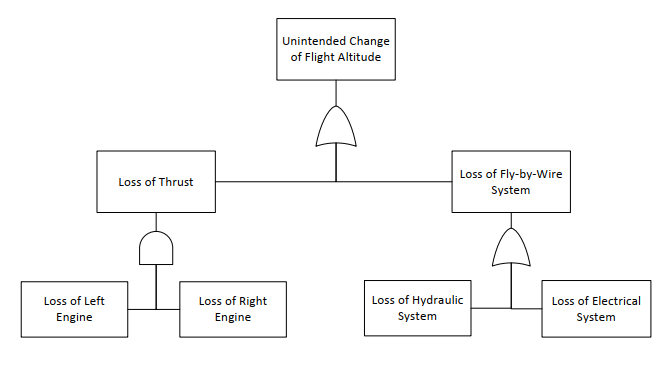
\includegraphics[width=9cm]{images/ft.png}
\caption{A Simple Fault Tree} \label{fig:introFT}
\end{center}
\end{figure}

Figure~\ref{fig:introFT} shows a simple example of a fault tree. In this example, the top level event corresponds to an aircraft having an unintended change of altitude. In order for this event to occur, there must be either a loss of thrust or the loss of a Fly-by-Wire system. This is seen through the use of the OR gate below the top level event. The malfunction of both the left and right engines will cause the loss of thrust to occur and the Fly-by-Wire system can be lost if either the hydraulic system or the electrical system were to malfunction. The MCSs for this example are \{Loss of Left Engine, Loss of Right Engine\}, \{Loss of Hydraulic System\}, and \{Loss of Electrical System\}. 

There are two main types of FTA that we differentiate here as \textit{qualitative} analysis and \textit{quantitative} analysis. In qualitative analysis, the structure of the fault tree is considered and the cut sets are a way to indicate which combinations of component failures will cause the system to fail. On the other hand, in quantitative analysis the probability of the TLE is calculated given the probability of occurance of the basic events. 


\subsubsection{Fault Mode and Effects Analysis}
FMEA is represented as a table that shows the relationships between sets of faults, intermediate events, and properties that represent undesirable states. Even though FMEA tables are different than fault trees, the generation of MCSs are often used to build the FMEA tables~\cite{Bozzano:2010:DSA:1951720}. For instance, the FMEA table in Figure~\ref{fig:introFMEA} represents the MCSs also found in the FT from Figure~\ref{fig:introFT}.

\begin{figure}[h]
\begin{center}
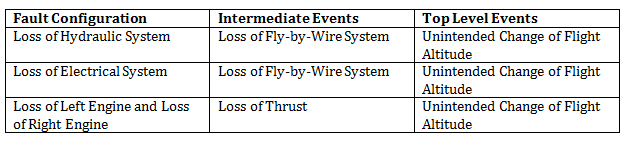
\includegraphics[width=9cm]{images/fmea.png}
\caption{A Simple FMEA Table} \label{fig:introFMEA}
\end{center}
\end{figure}

\subsubsection{Common Cause Analysis}
Common cause failure analysis attempts to find failures in the system for which two or more evens have the potential to occur due to the same cause. Some common causes include 


\subsubsection{Safety Artifacts in the MBSA Process}
The artifacts developed from the MBSA process can be updated iteratively from the shared nominal and fault model of the system. It is assumed that the model is created and maintained in sync with the hardware and software design and implementation and guided by the hazard and probability information from a preliminary system FTA. The analysis results for each iteration of the model are then used to update the preliminary system FTA. This process continues iteratively until the system safety property is satisfied with the desired fault tolerance and failure probability. 



